\documentclass[11pts]{report}

\usepackage{qtree}
\usepackage{listings}
\usepackage{amsmath,mathtools}
\usepackage[ruled,longend]{algorithm2e}
\usepackage{tikz}
\usepackage{listings}
\usepackage{graphicx}
\usepackage{xcolor}
\lstset{
    frame=tb, % draw a frame at the top and bottom of the code block
    tabsize=4, % tab space width
    showstringspaces=false, % don't mark spaces in strings
    commentstyle=\color{green}, % comment color
    keywordstyle=\color{blue}, % keyword color
    stringstyle=\color{red} % string color
}

\title{CS 677 Homework \\ Assignment 04}
\date{Semtember 26, 2018}
\author{Hai Nguyen}

\setlength{\topmargin}{-1cm}
\setlength{\oddsidemargin}{0in}
\setlength{\textwidth}{6.5in}
\setlength{\textheight}{8.3in}

\DeclareMathOperator{\Div}{div}
\newcommand{\vect}[1]{\mathbf{#1}}




%%Currently default settings for indentation and symbols.
%%Try these by uncommenting this block!!!
%%Redefine the first level symbols
%\renewcommand{\theenumi}{\fnsymbol{enumi}-}
%\renewcommand{\labelenumi}{\theenumi}
%
%%Redefine the second level symbols
%\renewcommand{\theenumii}{\alph{enumii})}
%\renewcommand{\labelenumii}{\theenumii}
%
%%Redefine the third level symbols
%\renewcommand{\theenumiii}{\roman{enumiii}.}
%\renewcommand{\labelenumiii}{\theenumiii}
%
%%Options for redefining levels


%\arabic
%\alph 
%\Alph
%\roman
%\Roman
%\fnsymbol
%This ^^^ is all you need to change!!

\begin{document}

\maketitle

\begin{enumerate}

% Question 1
\item Implement in C/C++ an algorithm to arrange elements of a given array of n real numbers so that all its negative elements precede all its positive elements. Show how your algorithm works on the following input: A = [4 3 -2 0 2 9 -1 10 0 5 23 -4].
\par \textit{Algorithm:} 
The algorithm will divide the array in 3 areas and there locations are in order: negative range, zero range and positive range. The algorithm starts with the zero range and this range will be widen to the left and right depending on the element it is examining. The algorithm has no need for a temporary array (memory space O(1)) and has the complexity O(n).
\par \textit{Implement in C++:}

\begin{lstlisting}

#include <stdio.h> 
  
void swap(int *xp, int *yp)
{
    int temp = *xp;
    *xp = *yp;
    *yp = temp;
}

void printArray(int arr[], int n) 
{ 
    for (int i = 0; i < n; i++) 
        printf("%d ", arr[i]); 
    printf("\n");
} 

void rearrange(int arr[], int n) 
{ 
    int negIdx  = 0;
    int zeroIdx = 0;
    int posIdx = n - 1;

    while (zeroIdx <= posIdx) {
        if (arr[zeroIdx] < 0)
        {
            swap(&arr[negIdx], &arr[zeroIdx]); 
            negIdx++; 
            zeroIdx++;

            printf("Negative Pass: ");
            printArray(arr, n);  
        }

        else if (arr[zeroIdx] == 0)
        {
            zeroIdx++;

            printf("Zero Pass:     ");
            printArray(arr, n);    
        }

        else
        {
            swap(&arr[posIdx], &arr[zeroIdx]); 
            posIdx--;

            printf("Positive Pass: ");
            printArray(arr, n);
        }
    }
}

  
int main() 
{ 
    int arr[] = { 4, 3, -2, 0, 2, 9, -1, 10, 0, 5, 23, -4 }; 
    int n = sizeof(arr) / sizeof(arr[0]); 
    rearrange(arr, n); 
    printf("\nSorted array: ");
    printArray(arr, n); 
    return 0; 
} 

\end{lstlisting}

\textit{Ouputs:}

\begin{lstlisting}
Positive Pass: -4 3 -2 0 2 9 -1 10 0 5 23 4 
Negative Pass: -4 3 -2 0 2 9 -1 10 0 5 23 4 
Positive Pass: -4 23 -2 0 2 9 -1 10 0 5 3 4 
Positive Pass: -4 5 -2 0 2 9 -1 10 0 23 3 4 
Positive Pass: -4 0 -2 0 2 9 -1 10 5 23 3 4 
Zero Pass:     -4 0 -2 0 2 9 -1 10 5 23 3 4 
Negative Pass: -4 -2 0 0 2 9 -1 10 5 23 3 4 
Zero Pass:     -4 -2 0 0 2 9 -1 10 5 23 3 4 
Positive Pass: -4 -2 0 0 10 9 -1 2 5 23 3 4 
Positive Pass: -4 -2 0 0 -1 9 10 2 5 23 3 4 
Negative Pass: -4 -2 -1 0 0 9 10 2 5 23 3 4 
Positive Pass: -4 -2 -1 0 0 9 10 2 5 23 3 4 

Sorted array: -4 -2 -1 0 0 9 10 2 5 23 3 4 
\end{lstlisting}


\item Answer the following question: is Quicksort a stable sorting algorithm? If yes, give a justification. If not, provide a counterexample.

\par Answer: \textit{Quicksort is unstable}
\par Counter example:
\par Given an input array: A = [0 2a 4 2b]. The input array have two equal keys - 2 elements of 2. They are differed by their labels 2a and 2b. If the sorting algorithm is stable then in the sorted output, the orders of equal keys will be maintained so 2a will precede 2b. Also when applying Quicksort as shown in Figure \ref{Fig:2}, we assume that we always take the final element in the array to be the pivot.

\begin{figure}[htbp]
\begin{center}
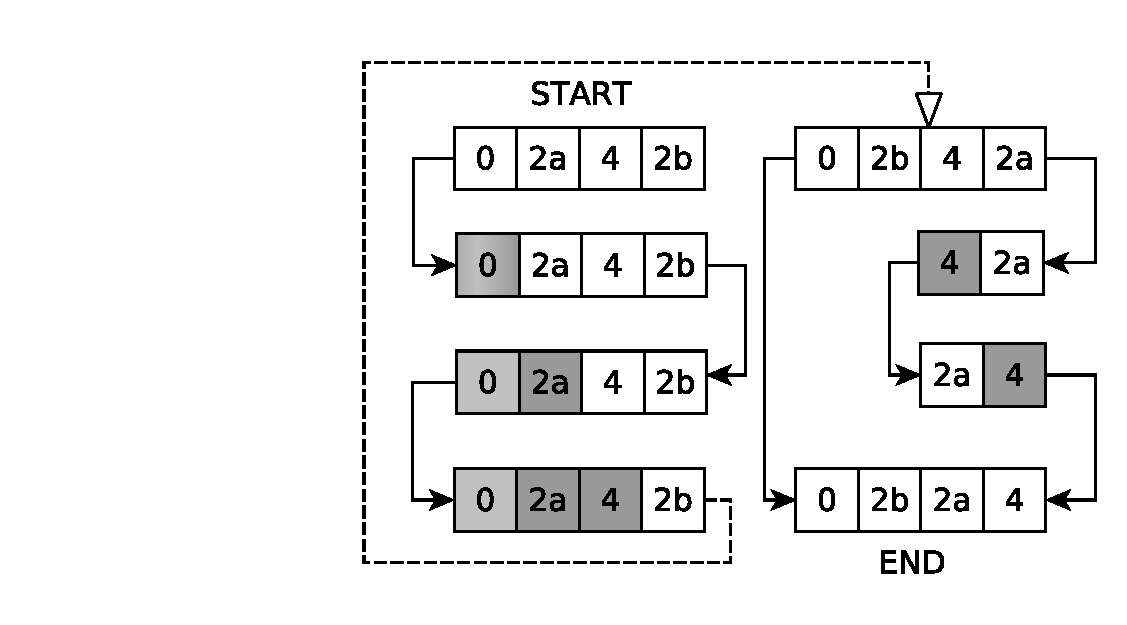
\includegraphics[scale=0.5]{21.pdf}
\caption{Counter example to prove that Quicksort is unstable.}
\label{Fig:2}
\end{center}
\end{figure}

Lightly shaded array elements are all in the first partition with values no greater than the pivot. Heavily shaded elements are in the second partition with values greater than the pivot. The unshaded elements have not yet been put in one of the first two partitions, and the final white element is the pivot. After we finish partitioning, in the sorted output array, we can see that the order between two equal keys (2a and 2b) are reversed, so Quicksort is not a stable algorithm.

\item 
\begin{enumerate}
\item Exercise 7.1-1 (page 173)
Illustrate the operation of PARTITION on the array A = [13, 19, 9, 5, 12, 8, 7, 4, 21, 2, 6, 11]

\begin{figure}[htbp]
\begin{center}
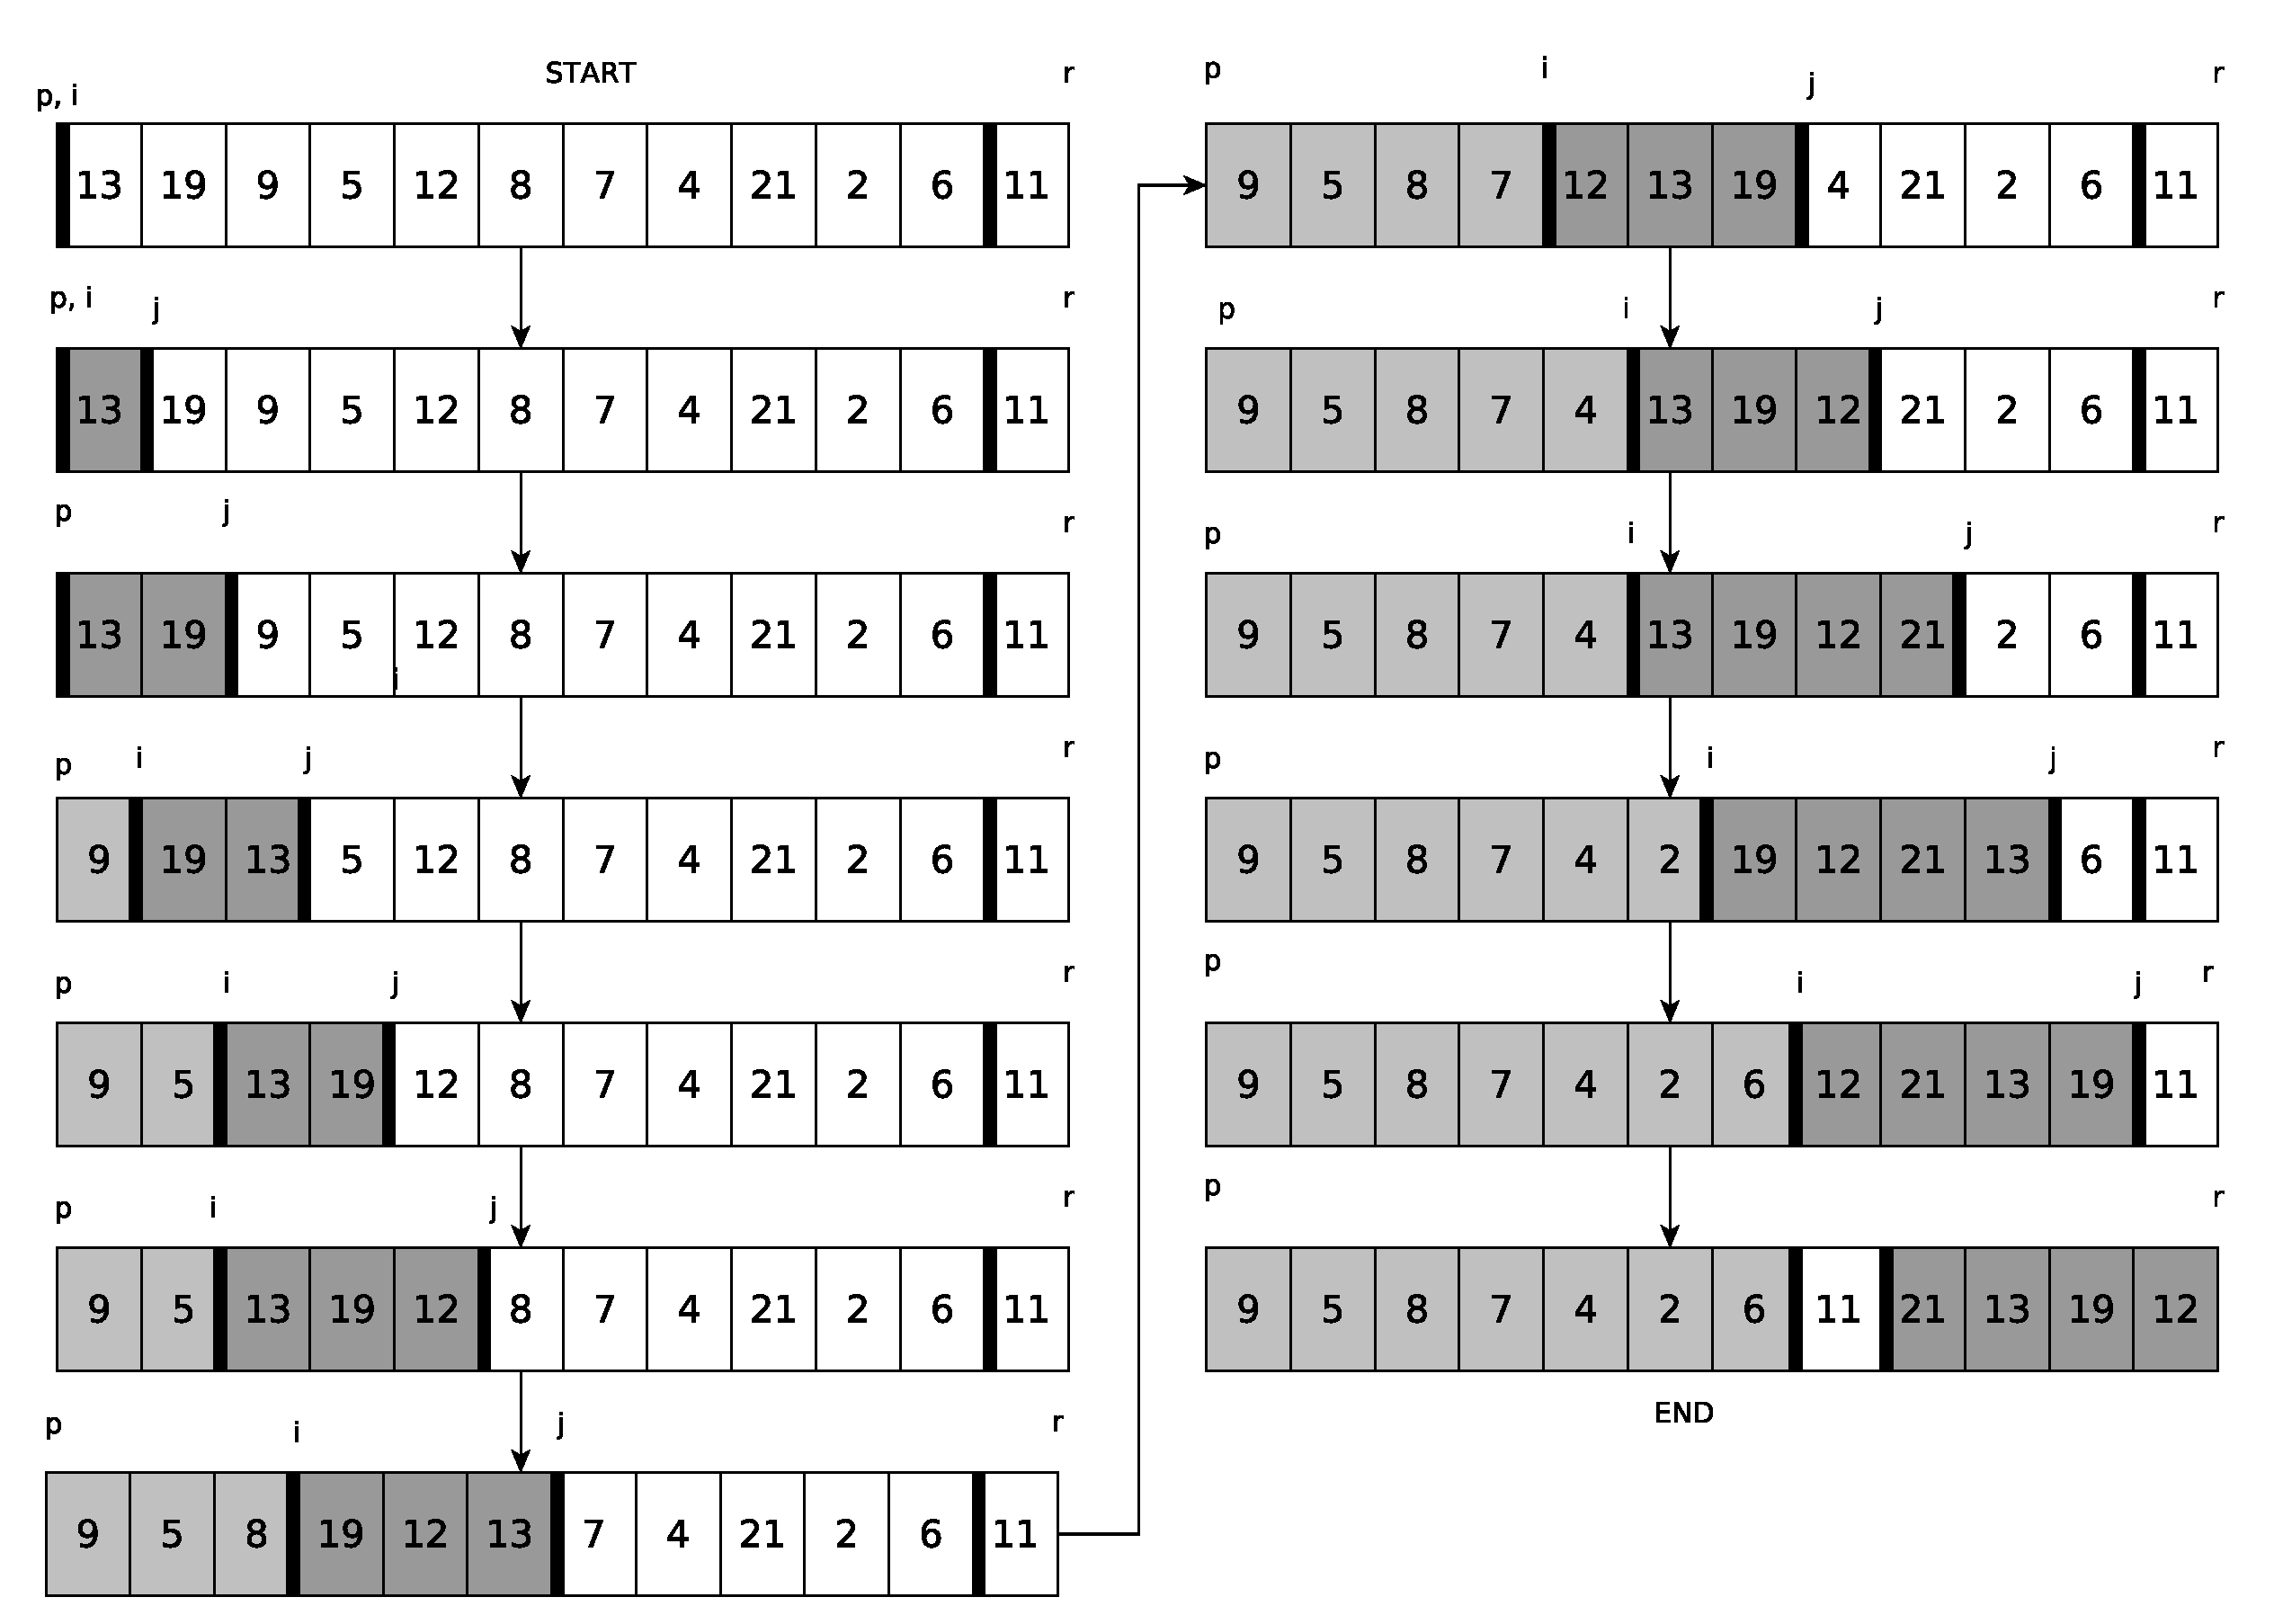
\includegraphics[scale=0.25]{3a.pdf}
\caption{Quicksort partitioning process.}
\label{Fig:5a}
\end{center}
\end{figure}

Figure \ref{Fig:5a} illustrates how partitioning is performed on the above array. Lightly shaded array elements are all in the first partition with values no greater than the pivot. Heavily shaded elements are in the second partition with values greater than the pivot. The unshaded elements have not yet been put in one of the first two partitions, and the final white element is the pivot.

\item Give an argument to show that RANDOMIZED-SELECT never makes a recursive call to a 0-length array.

\par \textbf{ALGORITHM}: RANDOMIZED-SELECT(A, p, r, i)
\par \textbf{if} p = r
\par \quad \textbf{then return} A[p]
\par q $\gets$ RANDOMIZED-PARTITION(A, p, r)
\par k $\gets$ q - p + 1
\par \textbf{if} i = k
\par \quad \textbf{then return } A[q]
\par \textbf{elseif} i $<$ k
\par \quad \textbf{then return} RANDOMIZED-SELECT(A, p, q - 1, i)
\par \textbf{else return} RANDOMIZED-SELECT(A, q + 1, r, i - k)

\par From the algorithm, RANDOMIZED-SELECT makes a recursive call to a 0-length array when:
\begin{itemize}
\item Line 8: p $>$ q - 1 $\to$ i $<$ k = q - p + 1 $\leq$ 1 $\to$ i = 0 (not possible - there is no such 0-th order statistic) 
\item Line 9: q + 1 $>$ r but because q $\leq$ r $\to$ q = r. However, in this case i $>$ k = q - p + 1 = r - p + 1 (number of elements in A) $\to$ i is not in A (not possible)
\end{itemize}
\par So the algorithm will never recurse on 0-length arrays.

\end{enumerate}

\item Exercise 9.3-5 (page 223). Suppose that you have a "black-box" worst-case linear-time median subroutine. Give a simple, linear-time algorithm that solves the selection problem for an arbitrary order statistic.
\par Algorithm to solve the selection problem for an i-order statistic in an input array A[1..n]:
\par \textbf{ALGORITHM} Select(A, i)
\par Median m $\gets$ Black-box median select for A [Time O(n)]
\par \textit{(We will get A1[1..n/2-1] and A2[n/2..n] by partitioning around the median m)}
\par \textbf{if} i = n/2 
\par \quad \textbf{return} A[n/2] [Time c1]
\par \textbf{elseif} i $<$ n/2
\par \quad \textbf{return} Select(A1, i) [Time T(n/2)]
\par \textbf{else return} Select(A2, n/2-i)  [Time T(n/2)]

Total time: 
\begin{align*}
T(n) &\leq cn + T(n/2) \\
      &\leq cn + T(n/2) \\
      &\leq cn(1 + \frac{1}{2} + ... + \frac{1}{2^m}) + T(1) \\
      &\leq cn\frac{1}{1-\frac{1}{2}} \\
      &\leq O(n)
\end{align*}

\item Exercise 9.2-4 (page 220). Suppose we use RANDOMIZED-SELECT to select the minimum element of the array A = [3, 2, 9, 0, 7, 5, 4, 8, 6, 1]. Describe a sequence of partitions that results in a worst-case performance of RANDOMIZED-SELECT.

The partitioning process is shown in Figure \ref{Fig:3a}. The worst case scenario is when RANDOMIZED-PARTITION keeps picking the maximum value in the array (number in shaded area) to be the pivot for partitioning. This results in the maximal unbalance between two partitioned arrays when one array is empty and (n - 1) remaining elements (including the minimum and excluding the pivot) are in the other array. Because all remaining elements are less than the pivot, the order of elements are kept after partitioning.

\begin{figure}[h]
\begin{center}
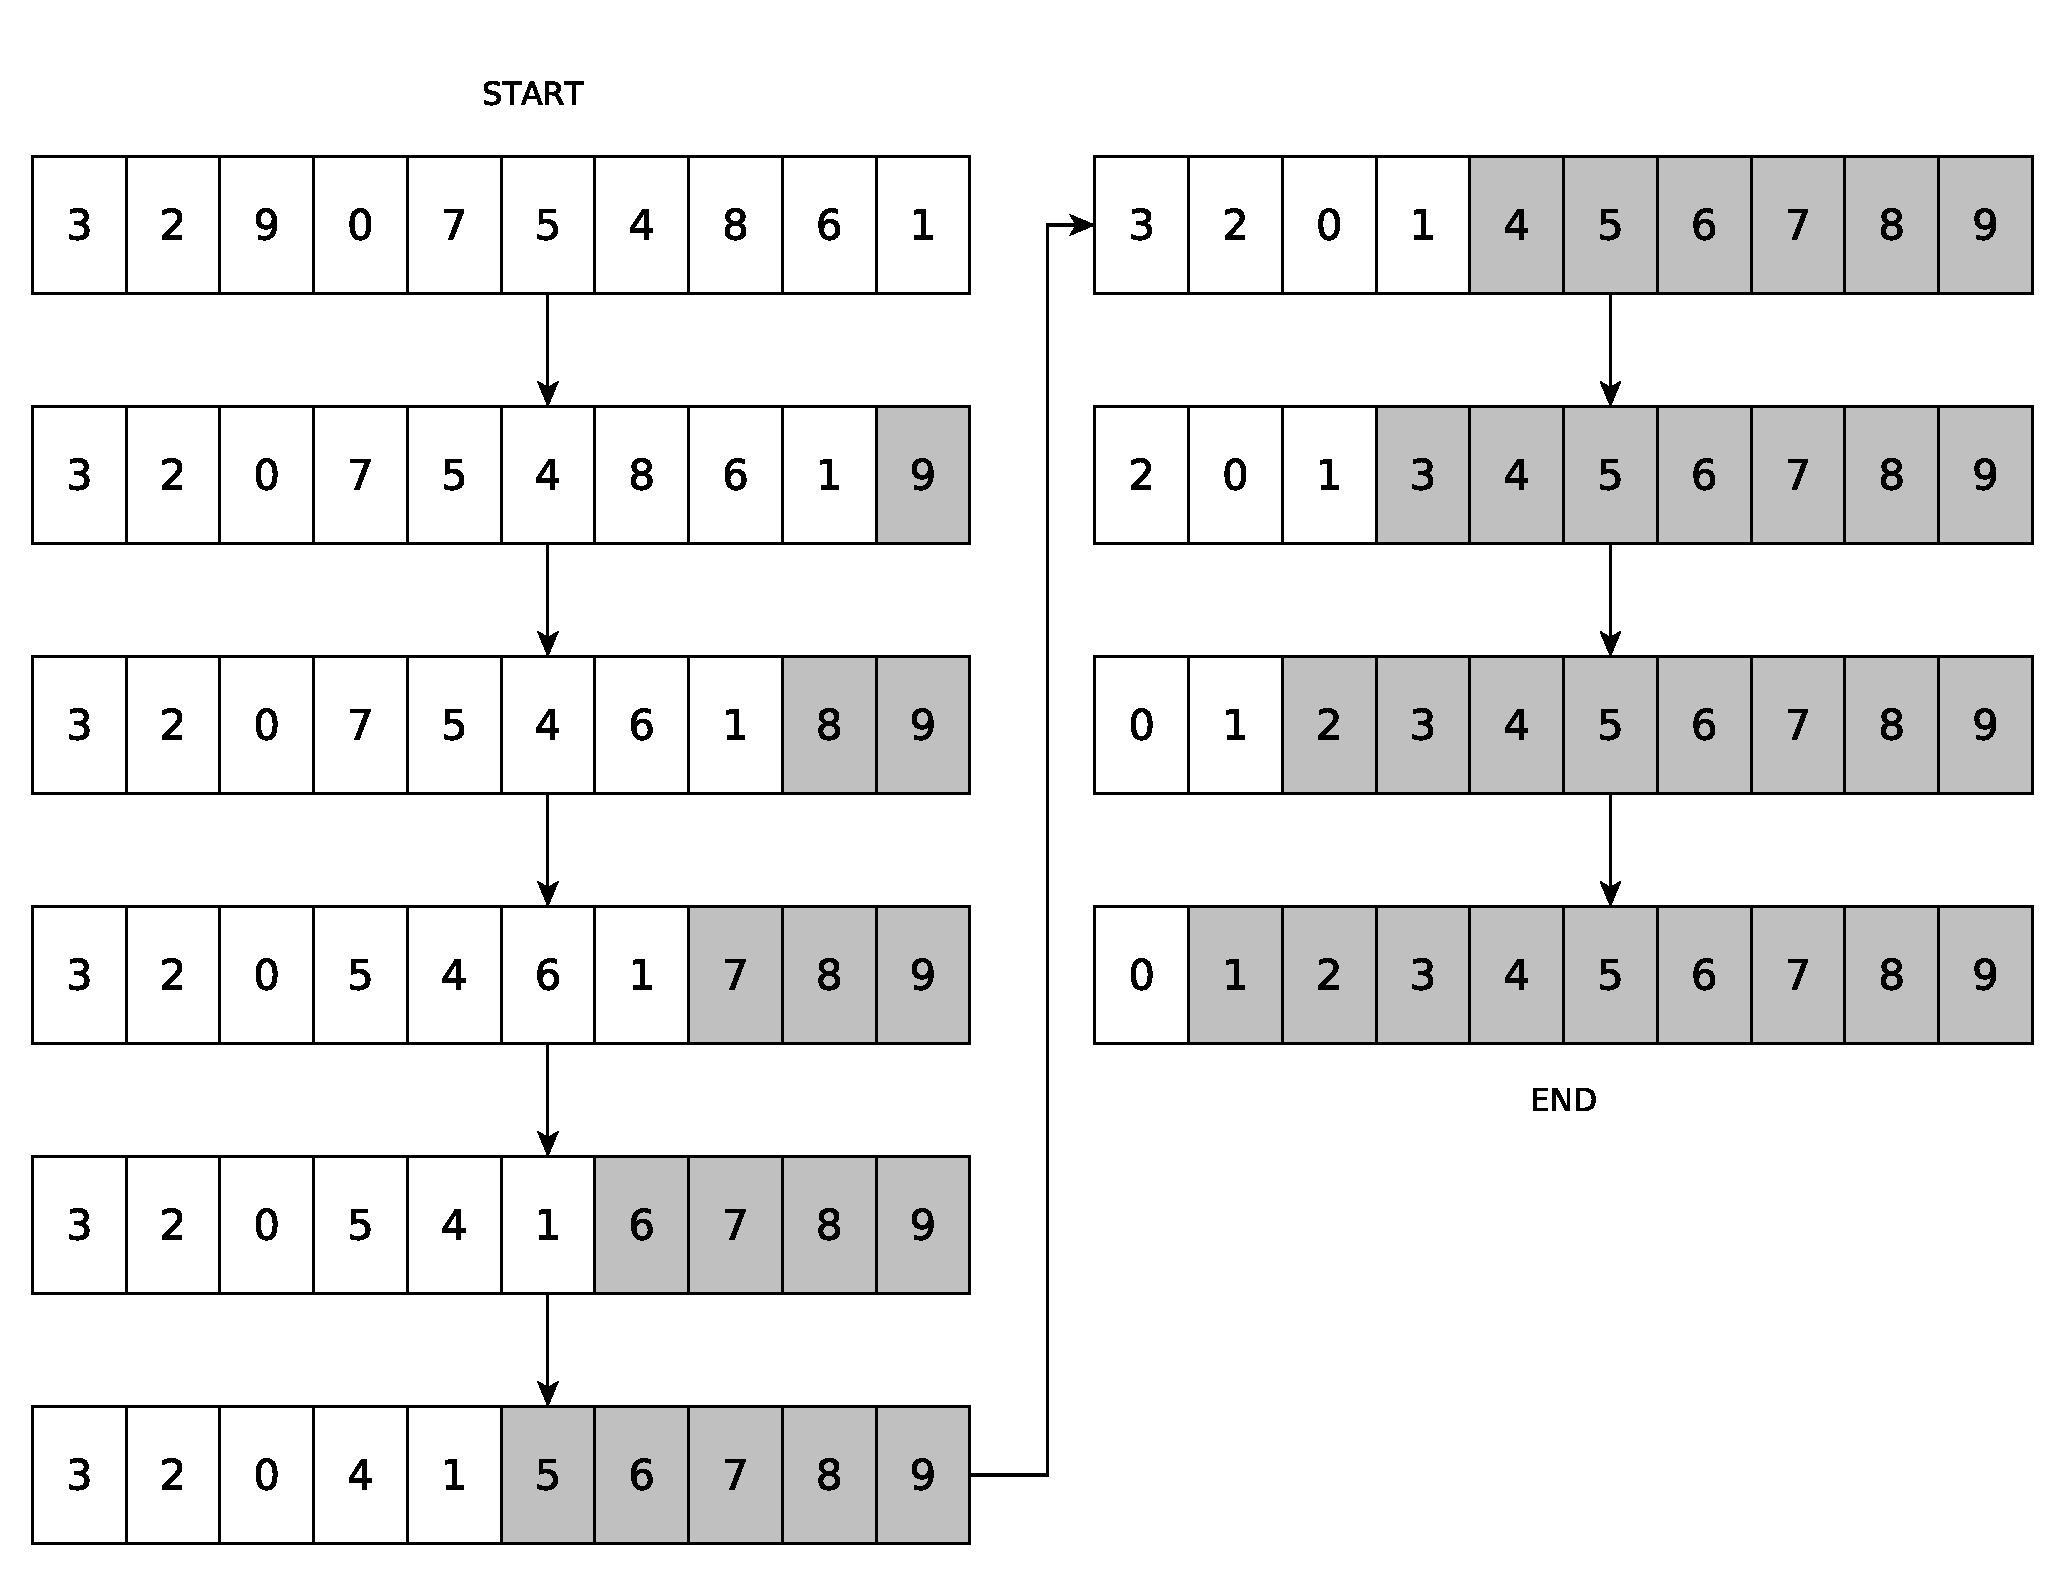
\includegraphics[scale=0.3]{5.pdf}
\caption{Worst case RANDOMIZED-SELECTION.}
\label{Fig:3a}
\end{center}
\end{figure}

\item Exercise 9.3-3 (page 223). Show how Quicksort can be made to run in O(nlgn) time in the worst case, assuming that all elements are distinct.

Using the Select algorithm mentioned in lecture, we can find the median of an array of distinct elements in linear time even in worst case. After that, we partition around the median value to get two arrays with equal number of elements. Then, we call Quicksort in these two arrays.

\par \textbf{ALGORITHM} Median-Quicksort(\textit{A})
\par Choose pivot to be the median of A $\gets$ Median select [Time O(n)]
\par \textit{(We will get A1[1..n/2-1] and A2[n/2..n] by partitioning around the median)}
\par \qquad Median-Quicksort(A1) [Time T(n/2)]
\par \qquad Median-Quickort(A2)  [Time T(n/2)]
\par
\par From the above algorithm, we have the recurrence relationship:
\begin{align*}
T(n) &= 2T(n/2) + O(n) \\
	 &= 2^{lgn}T(1) + (lgn - 1)O(n) \\
	 &= nT(1) + lgnO(n) \\
	 &= O(nlgn)
\end{align*}
So by using the selection algorithm to select the median in linear time even in worst case, we can use that strategy to replace the normal partition process to make Quicksort to run in O(nlgn) in the worst case.

\end{enumerate}

\end{document}
